\documentclass[conference]{IEEEtran}

\usepackage[english,spanish,es-noquoting]{babel}
\usepackage[utf8]{inputenc}
\usepackage[T1]{fontenc}
\usepackage{graphicx}
\usepackage{amsmath}
\usepackage{booktabs}
\usepackage{listings}
\usepackage{xcolor}
\usepackage{url}
\usepackage{hyperref}
\hypersetup{colorlinks=false, pdfborder={0 0 0}}

\graphicspath{{fig/}}

\lstset{
  basicstyle=\ttfamily\scriptsize,
  breaklines=true,
  columns=fullflexible,
  frame=single,
  framesep=3pt,
  numbers=none,
  showstringspaces=false,
  keywordstyle=\bfseries,
  language=Python,
}

\begin{document}

\title{FrostPuno: arquitectura distribuida y c\'omputo paralelo para la
predicci\'on de heladas mediante aprendizaje no supervisado en el altiplano
de Puno}

\author{
\IEEEauthorblockN{Mamani Mendoza, Joseph Elvis \quad Pari Pari, Yimmy Ronaldo
\quad Quispe Galindo, Jahan Kevin\\
Flores Curasi, H\'ector Luis \quad Apaza Llanos, Yoel}
\IEEEauthorblockA{Escuela Profesional de Ingenier\'ia de Sistemas\\
Universidad Nacional del Altiplano\\
Puno, Per\'u}
}

\maketitle

\renewcommand{\abstractname}{Abstract}
\begin{abstract}
\begin{otherlanguage}{english}
Frost events in the Peruvian highlands damage crops and cause neonatal mortality
in alpaca and sheep herds, yet the same frost is the essential input for
\emph{chu\~no}, a freeze-dried potato that sustains regional food security.
Producers currently decide when to protect crops or lay out potatoes based on
personal experience, without integrated climate information. This work presents
FrostPuno, a distributed system that groups the thermal regimes of thirteen
districts in Puno using K-Means and delivers the result as a live production
service. Three results are reported. First, the deployed system classifies all
thirteen districts into three risk levels with a silhouette coefficient of 0.419
and a Davies-Bouldin index of 0.813, and the resulting territorial ranking
matches regional geography without any hand-coded rule. Second, the system runs
in production at zero infrastructure cost, reachable as a web application, a
programming interface and an Android application, with automated retraining and
a quality gate whose blocking behaviour is verified by tests. Third, an economic
sustainability model is proposed, based on institutional licensing to local
governments and cooperatives, showing that the operation reaches break-even with
a small number of institutional subscribers. The parallel and distributed design
decisions that make this operating cost possible are described: thread-pool
ingestion with per-district fault isolation, four autonomous services coupled
only through explicit contracts, and concurrent continuous-integration jobs.
\end{otherlanguage}
\end{abstract}

\begin{IEEEkeywords}
parallel computing, distributed systems, unsupervised learning, K-Means,
continuous integration, frost prediction, economic sustainability, high-Andean
agriculture
\end{IEEEkeywords}

\renewcommand{\abstractname}{Resumen}
\begin{abstract}
FrostPuno agrupa los reg\'imenes t\'ermicos de trece distritos de Puno mediante
aprendizaje no supervisado y entrega el resultado como servicio en producci\'on,
accesible desde la web, una interfaz de programaci\'on y una aplicaci\'on
Android. El sistema clasifica los trece distritos en tres niveles de riesgo con
un coeficiente de silueta de 0.419, opera con costo de infraestructura nulo y se
mantiene solo mediante reentrenamiento programado con una barrera de calidad
verificada por pruebas. Se propone adem\'as un modelo de sostenibilidad
econ\'omica basado en licenciamiento institucional que alcanza el punto de
equilibrio con pocos suscriptores.
\end{abstract}

\section{Introducci\'on}

En la regi\'on Puno, por encima de los 3800 metros sobre el nivel del mar, las
heladas presentan una doble condici\'on. Da\~nan los cultivos y provocan
mortalidad neonatal en cr\'ias de alpaca y ovino, patrimonio productivo de las
familias altoandinas. Al mismo tiempo, constituyen el insumo indispensable del
chu\~no, papa deshidratada mediante congelamiento nocturno y secado diurno que
se conserva durante a\~nos y forma parte de la seguridad alimentaria regional.

La decisi\'on de proteger un cultivo, resguardar el ganado o tender la papa se
toma habitualmente por experiencia emp\'irica. No existe una herramienta que
integre informaci\'on clim\'atica abierta y la traduzca en recomendaciones
territoriales. El problema no se limita al modelado: exige recolectar datos de
m\'ultiples ubicaciones, servirlos con baja latencia a usuarios dispersos y
mantener el sistema operativo sin intervenci\'on constante.

Este art\'iculo describe FrostPuno desde la perspectiva del c\'omputo paralelo y
distribuido. Las contribuciones son las siguientes:

\begin{enumerate}
\item Una estrategia de ingesta paralela por hilos con aislamiento de fallos por
ubicaci\'on, adecuada a una carga dominada por latencia de red.
\item Una arquitectura distribuida en cuatro servicios aut\'onomos, desplegados
en proveedores distintos y acoplados \'unicamente por contratos expl\'icitos.
\item Un esquema de mantenimiento automatizado del componente inteligente,
ejecutado como trabajos concurrentes de integraci\'on continua y protegido por
una barrera de calidad verificada mediante pruebas.
\end{enumerate}

\section{Trabajos relacionados}

La predicci\'on de heladas se ha abordado tradicionalmente con modelos
supervisados que requieren registros hist\'oricos etiquetados de eventos
ocurridos. En territorios donde esos registros no existen o no son accesibles de
forma program\'atica, el agrupamiento ofrece una alternativa: permite descubrir
reg\'imenes clim\'aticos sin necesidad de etiquetas.

En cuanto a la operaci\'on de sistemas con componentes de aprendizaje, la
pr\'actica de separar el entrenamiento por lotes de la inferencia en l\'inea, y
de intermediar ambos mediante un registro de modelos, se ha consolidado como
patr\'on de referencia. FrostPuno adopta ese patr\'on y lo complementa con una
barrera de calidad que impide promover modelos degradados, aspecto que suele
quedar fuera de los trabajos acad\'emicos de alcance similar.

\section{Arquitectura distribuida}

El sistema se descompone en cuatro servicios aut\'onomos que se comunican por
HTTP siguiendo contratos REST estables. Cada uno reside en una plataforma
distinta, de modo que la distribuci\'on es efectiva y no una separaci\'on
l\'ogica dentro de un mismo proceso.

\begin{table}[htbp]
\caption{Distribuci\'on de los componentes del sistema}
\begin{center}
\begin{tabular}{@{}lll@{}}
\toprule
\textbf{Componente} & \textbf{Plataforma} & \textbf{Responsabilidad} \\
\midrule
Cliente Flutter & Vercel, APK & Presentaci\'on, ubicaci\'on \\
Servicio FastAPI & Render & Inferencia y reglas \\
Base de datos & Supabase & Persistencia \\
Fuente clim\'atica & Open-Meteo & Datos externos \\
\bottomrule
\end{tabular}
\label{tab:arquitectura}
\end{center}
\end{table}

El desacoplamiento se sostiene en dos decisiones. La primera es que el cliente
conoce \'unicamente la direcci\'on del servicio, inyectada en tiempo de
compilaci\'on, por lo que el mismo c\'odigo fuente produce la versi\'on web, la
versi\'on de desarrollo y la aplicaci\'on Android. La segunda es que el servicio
organiza su c\'odigo en capas sucesivas de rutas, servicios y repositorios, lo
que permite sustituir la persistencia sin alterar los controladores.

\begin{figure}[htbp]
\centerline{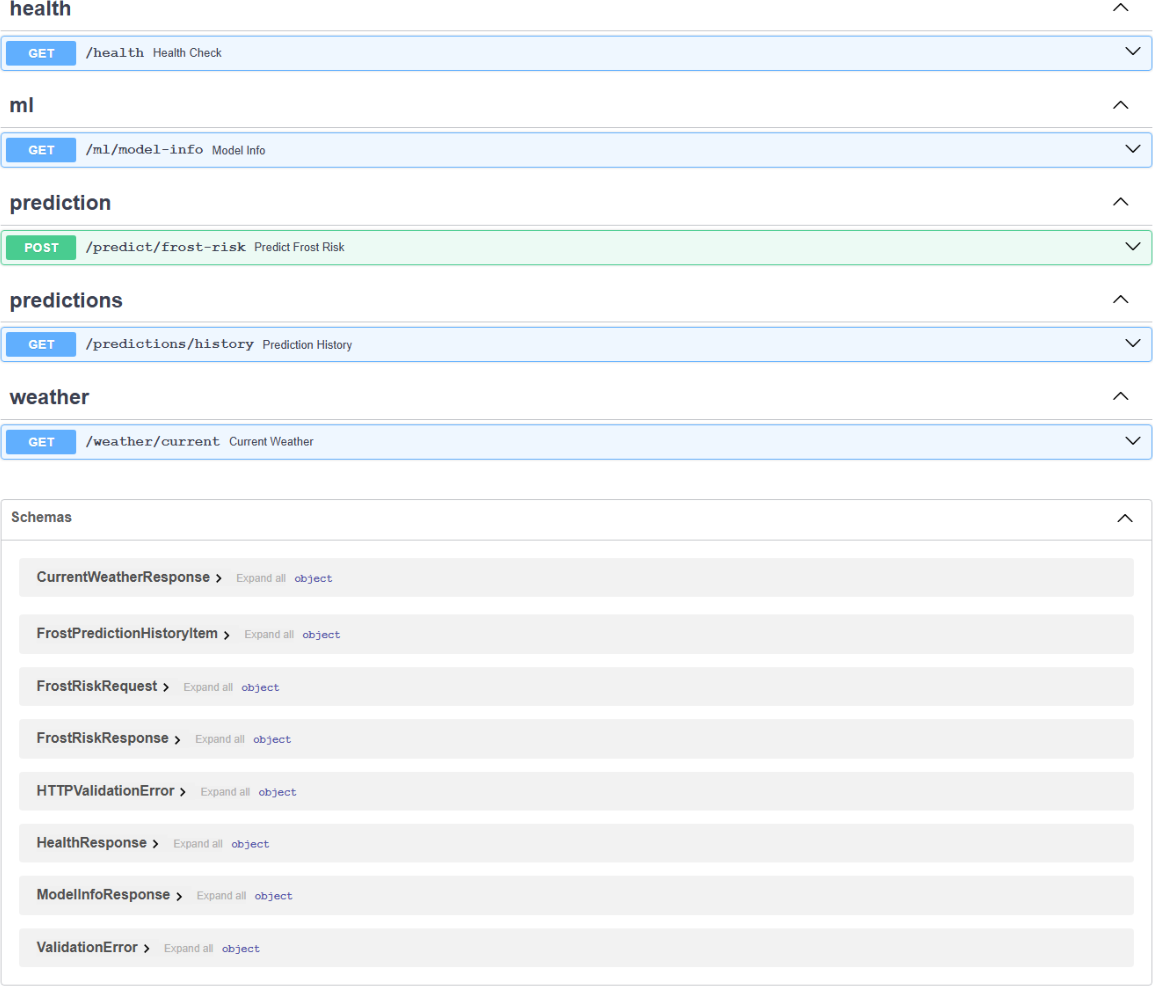
\includegraphics[width=0.47\textwidth]{swagger_api}}
\caption{Contrato REST publicado por el servicio en producci\'on.}
\label{fig:swagger}
\end{figure}

\section{Paralelismo en la ingesta de datos}

La construcci\'on del conjunto de datos requiere recolectar series clim\'aticas
horarias para trece distritos. Cada solicitud es independiente y su costo
est\'a dominado por la latencia de red, no por el procesador, de modo que la
carga es adecuada para paralelismo por hilos.

El listado \ref{lst:ingesta} muestra la implementaci\'on. Se lanzan tantas
tareas como distritos y se recolectan conforme finalizan, sin respetar el orden
de emisi\'on.

\begin{lstlisting}[caption={Ingesta paralela con aislamiento de fallos},label={lst:ingesta}]
with ThreadPoolExecutor(max_workers=max_workers) as executor:
    futures = {
        executor.submit(fetch_weather_for_location,
                        record, start_date, end_date): record
        for record in records
    }
    for future in as_completed(futures):
        record = futures[future]
        try:
            frames.append(future.result())
        except Exception as exc:
            failures.append(
                f"{record['ubigeo']} {record['distrito']}: {exc}")
\end{lstlisting}

Se destacan cuatro propiedades. La primera es el patr\'on de dispersi\'on y
recolecci\'on: la construcci\'on del diccionario de tareas dispersa el trabajo y
la iteraci\'on sobre las tareas completadas lo recolecta a medida que concluye.
La segunda es el aislamiento de fallos: la captura de excepciones se realiza por
tarea, de manera que la indisponibilidad de un distrito no interrumpe la
recolecci\'on de los restantes y queda registrada de forma individual. La tercera
es que el grado de paralelismo es configurable mediante un par\'ametro,
ajustable seg\'un el ancho de banda disponible y las restricciones del proveedor
de datos. La cuarta se refiere al rendimiento: siendo la carga dependiente de
entrada y salida, el tiempo total tiende al de una sola solicitud en lugar del
producto del n\'umero de distritos por ese tiempo, comportamiento consistente
con la fracci\'on paralelizable descrita por la ley de Amdahl.

\section{Distribuci\'on del c\'omputo de aprendizaje}

El sistema separa el c\'omputo intensivo del c\'omputo sensible a la latencia,
siguiendo el patr\'on habitual en sistemas distribuidos de aprendizaje
autom\'atico.

El entrenamiento se ejecuta por lotes y fuera de l\'inea. Recorre una
b\'usqueda exhaustiva de veinticuatro combinaciones de hiperpar\'ametros y
serializa el resultado en un registro de modelos junto con sus metadatos. La
inferencia, en cambio, ocurre en l\'inea: el servicio carga ese mismo artefacto
una \'unica vez por proceso y, ante cada solicitud, asigna el vector clim\'atico
al centroide m\'as pr\'oximo, operaci\'on de costo proporcional al n\'umero de
grupos y por tanto muy econ\'omica.

La pieza que articula ambos extremos es la lista de caracter\'isticas declarada
en los metadatos. El servicio construye el vector de entrada siguiendo ese
orden, por lo que un reentrenamiento no obliga a modificar el c\'odigo del
servidor. Este contrato constituye la frontera entre el subsistema de
aprendizaje y el subsistema de servicio.

Adicionalmente, el servicio incorpora tres mecanismos de eficiencia. Emplea un
servidor concurrente que atiende m\'ultiples solicitudes simult\'aneas; mantiene
una cach\'e en memoria indexada por coordenada con tiempo de expiraci\'on, lo
que evita consultar la fuente externa de forma repetida; e instancia una sola
vez por proceso el registro de modelos, el servicio de predicci\'on y el
proveedor clim\'atico, evitando recargar el artefacto serializado en cada
solicitud.

\section{Modelo de agrupamiento}

\subsection{Conjunto de datos y caracter\'isticas}

La fuente clim\'atica es Open-Meteo, de la que se obtienen series horarias para
trece distritos, resultando un conjunto de 4368 registros. La informaci\'on
territorial procede de una semilla compatible con el Instituto Nacional de
Estad\'istica e Inform\'atica.

Se parti\'o de ocho variables clim\'aticas. Un experimento de subconjuntos
evidenci\'o que la precipitaci\'on, la velocidad del viento, la nubosidad y la
temperatura aparente introduc\'ian ruido o resultaban colineales, degradando la
separaci\'on entre grupos. Al retirarlas, el coeficiente de silueta ascendi\'o
de 0.286 a 0.419, una mejora cercana al 47 por ciento obtenida mediante
reducci\'on y no mediante incorporaci\'on de informaci\'on. Las cuatro
caracter\'isticas conservadas son la altitud estimada, la temperatura, el punto
de roc\'io y la humedad relativa.

\subsection{Optimizaci\'on de hiperpar\'ametros}

El algoritmo es K-Means, precedido por un escalado estandarizado necesario dado
que las variables presentan magnitudes heterog\'eneas. La configuraci\'on se
determin\'o mediante b\'usqueda exhaustiva que maximiza el coeficiente de
silueta.

\begin{table}[htbp]
\caption{Espacio de b\'usqueda y configuraci\'on seleccionada}
\begin{center}
\begin{tabular}{@{}lll@{}}
\toprule
\textbf{Hiperpar\'ametro} & \textbf{Valores} & \textbf{Elegido} \\
\midrule
N\'umero de grupos & 3 a 8 & 3 \\
Inicializaci\'on & k-means++, aleatoria & aleatoria \\
Reinicios & 10, 25 & 10 \\
Semilla & fija & 42 \\
\bottomrule
\end{tabular}
\label{tab:hiperparametros}
\end{center}
\end{table}

\subsection{Evaluaci\'on}

Al tratarse de aprendizaje no supervisado no se dispone de etiquetas de
referencia, por lo que no procede el uso de exactitud ni de la medida F1. La
evaluaci\'on cuantifica la calidad de la estructura descubierta.

\begin{table}[htbp]
\caption{Selecci\'on del n\'umero de grupos}
\begin{center}
\begin{tabular}{@{}lcc@{}}
\toprule
\textbf{Grupos} & \textbf{Silueta} & \textbf{Davies-Bouldin} \\
\midrule
3 (elegido) & 0.4195 & 0.813 \\
4 & 0.3894 & 0.906 \\
5 & 0.3760 & 0.820 \\
6 & 0.3697 & 0.870 \\
7 & 0.3645 & 0.865 \\
8 & 0.3391 & 0.883 \\
\bottomrule
\end{tabular}
\label{tab:seleccion}
\end{center}
\end{table}

La configuraci\'on de tres grupos resulta superior en ambas medidas y coincide
con los tres niveles de riesgo que requiere la aplicaci\'on. La asignaci\'on de
niveles se realiza con posterioridad al entrenamiento, ordenando los grupos por
su temperatura media: el m\'as fr\'io corresponde al riesgo alto. Se trata de
una descripci\'on de los grupos hallados y no de una supervisi\'on, dado que el
entrenamiento no accede a esas etiquetas.

El resultado admite interpretaci\'on geogr\'afica. El distrito de Macusani,
situado a 4315 metros, queda clasificado en riesgo alto, mientras que Sandia,
ubicado en valle a 2170 metros, corresponde al riesgo bajo. Esta
correspondencia con la geograf\'ia regional emerge del agrupamiento y no fue
codificada mediante reglas.

\begin{figure}[htbp]
\centerline{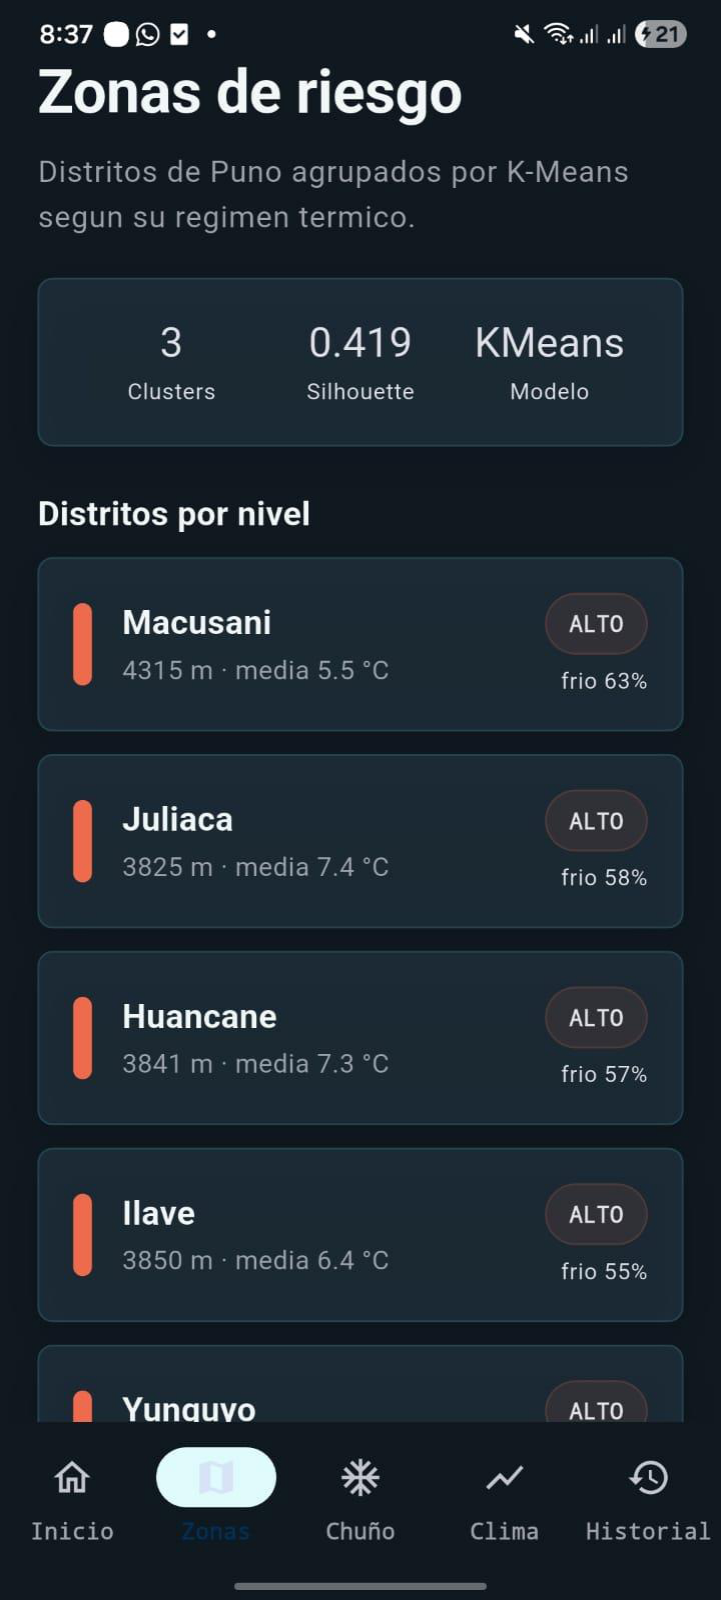
\includegraphics[width=0.24\textwidth]{zonas_kmeans}}
\caption{Agrupamiento de distritos con las m\'etricas del modelo en producci\'on.}
\label{fig:zonas}
\end{figure}

\section{Mantenimiento e integraci\'on continua}

El mantenimiento de un sistema con componentes de aprendizaje no se limita al
c\'odigo. Comprende el reentrenamiento, el registro de versiones, el
almacenamiento de caracter\'isticas y el control de calidad previo a la
promoci\'on de un modelo.

\subsection{Trabajos concurrentes}

Se implementaron cinco flujos independientes que se ejecutan de forma
simult\'anea en entornos aislados ante cada incorporaci\'on de cambios. El
primero entrena el modelo y publica los artefactos; el segundo aplica la barrera
de calidad y ejecuta las pruebas de mantenimiento; el tercero verifica el
servicio; el cuarto valida los conjuntos de datos; y el quinto analiza y compila
el cliente. Al no existir dependencias entre ellos, el tiempo total corresponde
al del flujo m\'as lento y no a la suma de todos.

\begin{figure}[htbp]
\centerline{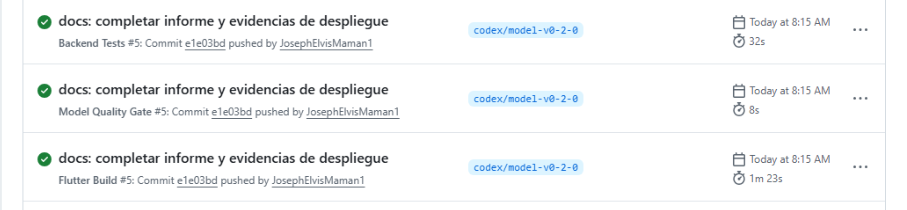
\includegraphics[width=0.47\textwidth]{actions_detalle}}
\caption{Ejecuciones concurrentes de los flujos de integraci\'on continua.}
\label{fig:actions}
\end{figure}

\subsection{Reentrenamiento adaptativo}

El flujo de entrenamiento cuenta con una programaci\'on semanal, por lo que el
modelo incorpora datos recientes sin intervenci\'on humana. El procedimiento no
se limita a repetir el entrenamiento: si la calidad obtenida no alcanza el
objetivo definido, ampl\'ia la ventana de datos hist\'oricos de catorce a
veintinueve y luego a cuarenta y cuatro d\'ias, y reintenta. Cada ejecuci\'on se
registra en un historial que documenta la evoluci\'on de la calidad frente al
volumen de datos disponible.

\subsection{Barrera de calidad}

El reentrenamiento autom\'atico introduce el riesgo de promover un modelo
inferior al vigente. Para evitarlo se verifica el coeficiente de silueta antes
de cualquier promoci\'on; si el valor se sit\'ua por debajo de 0.35, el proceso
finaliza con c\'odigo de error y la integraci\'on se detiene.

La existencia de la barrera no demuestra por s\'i sola su funcionamiento. Se
implementaron seis pruebas automatizadas que se ejecutan dentro de la
integraci\'on continua y verifican el ciclo completo: la generaci\'on de
artefactos, la capacidad de carga e inferencia del modelo serializado, la
cobertura territorial, la documentaci\'on de la b\'usqueda de hiperpar\'ametros,
la aprobaci\'on del modelo vigente y, de manera particular, el rechazo de un
modelo deliberadamente degradado. Esta \'ultima prueba construye un conjunto de
metadatos con una medida insuficiente y comprueba que el control lo bloquea.

\section{Resultados}

\subsection{Resultado territorial}

El sistema clasifica los trece distritos evaluados en tres niveles de riesgo. El
ordenamiento coincide con la geograf\'ia regional sin haber sido codificado:
Macusani, a 4315 metros, resulta de riesgo alto, mientras que Sandia, ubicado en
valle a 2170 metros, resulta de riesgo bajo. Esa correspondencia es el resultado
m\'as relevante del trabajo, porque indica que la estructura descubierta por el
agrupamiento tiene sentido f\'isico y no es un artefacto del procedimiento.

\begin{table}[htbp]
\caption{Clasificaci\'on territorial obtenida}
\begin{center}
\begin{tabular}{@{}lccc@{}}
\toprule
\textbf{Nivel} & \textbf{Distritos} & \textbf{Temp. media} & \textbf{Altitud media} \\
\midrule
Alto & 6 & 4.0 $^\circ$C & 3905 m \\
Medio & 6 & 11.6 $^\circ$C & 3893 m \\
Bajo & 1 & 13.6 $^\circ$C & 2170 m \\
\bottomrule
\end{tabular}
\label{tab:territorio}
\end{center}
\end{table}

\subsection{Producto en operaci\'on}

El sistema no es un prototipo de laboratorio: opera de forma p\'ublica y
continua. La tabla \ref{tab:resultados} resume las verificaciones.

\begin{table}[htbp]
\caption{Verificaciones sobre el sistema desplegado}
\begin{center}
\begin{tabular}{@{}ll@{}}
\toprule
\textbf{Verificaci\'on} & \textbf{Resultado} \\
\midrule
Canales de acceso & Web, API y Android \\
Costo de infraestructura & 0 USD mensuales \\
Pruebas del servicio & 12 satisfactorias \\
Pruebas de mantenimiento & 6 satisfactorias \\
Barrera de calidad & Aprobada, 0.419 \\
Intervenci\'on humana requerida & Ninguna \\
Modelo en producci\'on & K-Means v1.0.0 \\
\bottomrule
\end{tabular}
\label{tab:resultados}
\end{center}
\end{table}

Dos cifras de esa tabla concentran el valor pr\'actico del dise\~no. La primera
es el \textbf{costo cero} de operaci\'on, consecuencia directa de haber distribuido el
sistema en servicios que caben en los planes gratuitos de cada proveedor. La
segunda es que el sistema \textbf{no requiere intervenci\'on humana}: el
reentrenamiento ocurre por programaci\'on y la barrera de calidad decide si el
modelo nuevo se promueve. Ambas condiciones son las que hacen viable el modelo
econ\'omico que se describe en la secci\'on siguiente.

\begin{figure}[htbp]
\centerline{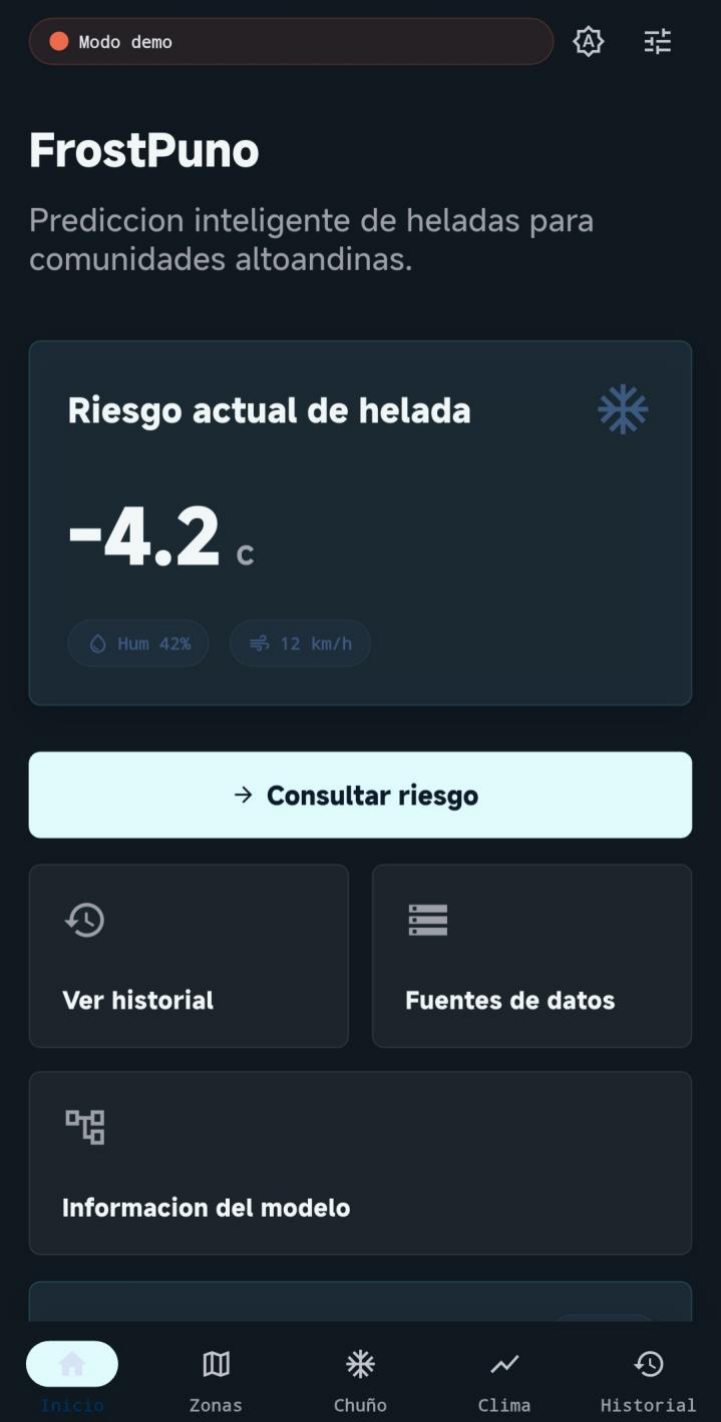
\includegraphics[width=0.22\textwidth]{home_oscuro}
\hfil
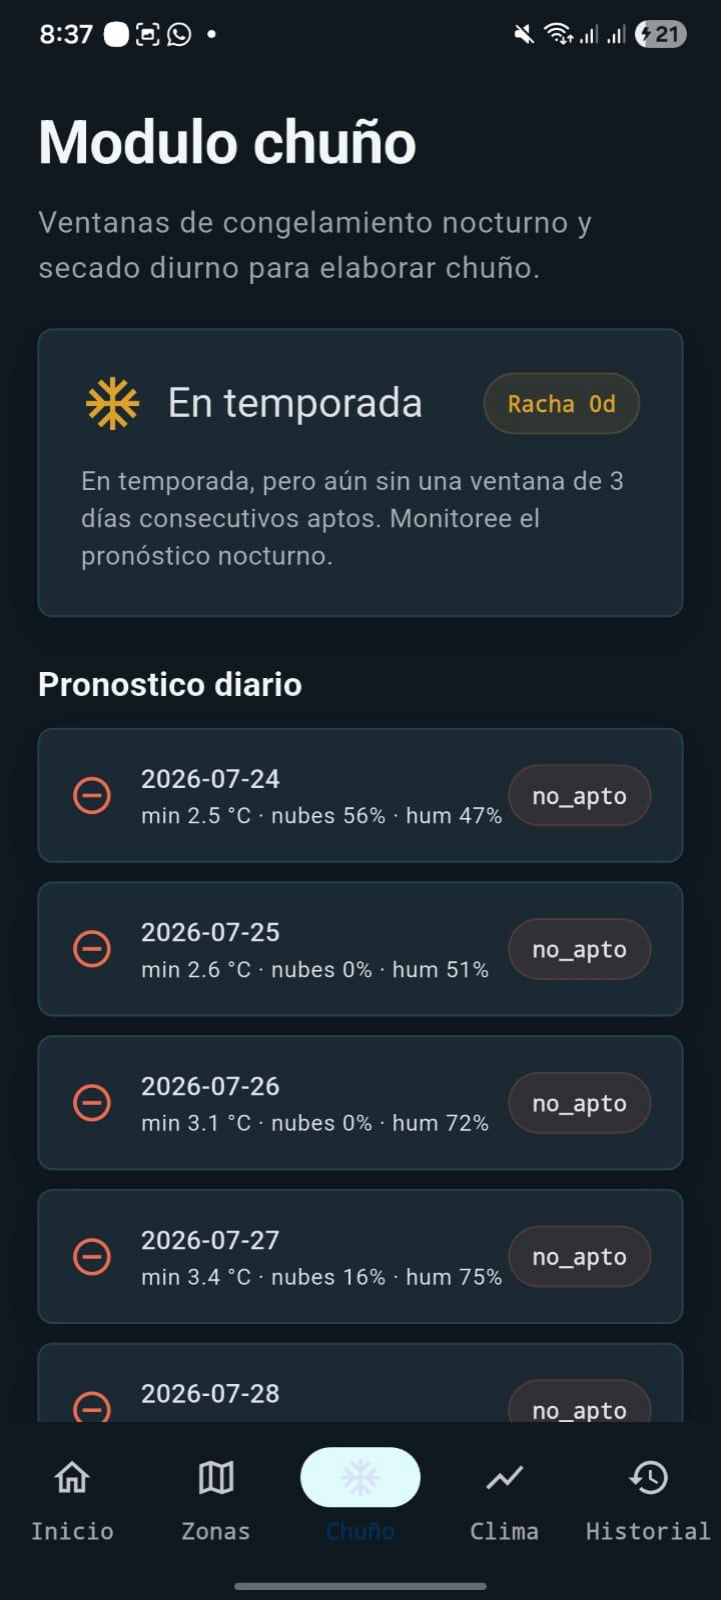
\includegraphics[width=0.22\textwidth]{chuno}}
\caption{Cliente en operaci\'on: alerta diaria y m\'odulo estacional de chu\~no.}
\label{fig:app}
\end{figure}

\subsection{Funcionalidad entregada al usuario}

La aplicaci\'on traduce la salida del modelo en decisiones concretas: alerta
diaria de helada con umbral configurable por el propio usuario, aviso
diferenciado para ganado orientado a la protecci\'on de cr\'ias, detecci\'on de
eventos inusuales frente a la climatolog\'ia reciente, agrupamiento territorial,
m\'odulo estacional de chu\~no e hist\'orico clim\'atico. Incorpora selecci\'on
de idioma entre espa\~nol e ingl\'es.

\section{Sostenibilidad econ\'omica}

Un sistema desplegado solo permanece \'util si puede sostenerse en el tiempo.
Esta secci\'on presenta la estructura de costos verificada y un modelo de
ingresos proyectado. Se distingue expl\'icitamente entre ambos: los costos
corresponden a la operaci\'on actual y son verificables; los ingresos son una
proyecci\'on sujeta a las suposiciones que se declaran.

\subsection{Estructura de costos verificada}

La decisi\'on de distribuir el sistema en servicios peque\~nos y aut\'onomos
tiene una consecuencia econ\'omica directa: cada componente cabe en el plan
gratuito de su proveedor. El costo operativo actual es nulo.

\begin{table}[htbp]
\caption{Costo mensual de operaci\'on (USD aproximados)}
\begin{center}
\begin{tabular}{@{}lcc@{}}
\toprule
\textbf{Componente} & \textbf{Actual} & \textbf{Plan pagado} \\
\midrule
Servicio backend & 0 & 7 \\
Cliente web & 0 & 20 \\
Base de datos & 0 & 25 \\
Integraci\'on continua & 0 & 0 \\
Fuente clim\'atica & 0 & 0 \\
\midrule
\textbf{Total} & \textbf{0} & \textbf{52} \\
\bottomrule
\end{tabular}
\label{tab:costos}
\end{center}
\end{table}

El escenario de plan pagado corresponde a precios p\'ublicos aproximados de los
proveedores y ser\'ia necesario \'unicamente al superar los l\'imites del nivel
gratuito, principalmente por volumen de usuarios concurrentes. La ausencia de
servidores propios elimina adem\'as el costo de administraci\'on de
infraestructura, que en un despliegue tradicional suele superar al costo del
propio servicio.

\subsection{Modelo de ingresos propuesto}

El usuario final directo es el productor altoandino, para quien el pago
individual no es viable ni deseable. El modelo propuesto mantiene la aplicaci\'on
gratuita para el productor y traslada el ingreso a las instituciones que se
benefician de la informaci\'on agregada.

\begin{table}[htbp]
\caption{L\'ineas de ingreso propuestas}
\begin{center}
\begin{tabular}{@{}p{2.1cm}p{2.6cm}p{2.4cm}@{}}
\toprule
\textbf{L\'inea} & \textbf{Cliente} & \textbf{Propuesta de valor} \\
\midrule
Licencia institucional &
Municipalidades y gobierno regional &
Panel de riesgo por distrito para dirigir campa\~nas de prevenci\'on \\
\addlinespace
Suscripci\'on asociativa &
Cooperativas y asociaciones de productores &
Alertas y ventanas de chu\~no para sus asociados \\
\addlinespace
Servicio de datos &
Aseguradoras agrarias &
Historial de riesgo territorial para tarificaci\'on \\
\addlinespace
Convenio &
Entidades p\'ublicas del sector &
Cobertura ampliada y validaci\'on de campo \\
\bottomrule
\end{tabular}
\label{tab:ingresos}
\end{center}
\end{table}

\subsection{Punto de equilibrio}

Bajo el escenario de plan pagado de la tabla \ref{tab:costos}, el costo
operativo anual asciende a unos 624 d\'olares. Suponiendo una licencia
institucional anual de 500 d\'olares por municipalidad, cifra deliberadamente
conservadora frente al presupuesto de una campa\~na de prevenci\'on de heladas,
el punto de equilibrio se alcanza con \textbf{dos} entidades suscritas. La provincia
de Puno agrupa m\'as de una decena de municipalidades distritales, de modo que
el umbral se sit\'ua muy por debajo del mercado potencial inmediato.

El costo marginal de incorporar una entidad adicional es pr\'acticamente nulo,
porque el sistema ya calcula el agrupamiento de todos los distritos en la misma
ejecuci\'on. Esa asimetr\'ia entre costo fijo bajo y costo marginal nulo es la
que otorga viabilidad al modelo.

\subsection{Condiciones para la rentabilidad}

Tres decisiones t\'ecnicas del trabajo son las que sostienen esta viabilidad y
conviene se\~nalarlas de forma expl\'icita:

\begin{itemize}
\item La \textbf{arquitectura distribuida} permite que cada componente permanezca
dentro de un plan gratuito, lo que reduce el costo fijo a cero durante la etapa
de validaci\'on.
\item El \textbf{mantenimiento automatizado} elimina el costo recurrente de personal
dedicado a reentrenar y verificar el modelo, que en un sistema de aprendizaje
suele ser el gasto dominante.
\item La \textbf{ingesta paralela} mantiene el tiempo de actualizaci\'on acotado al
incorporar nuevos distritos, de modo que ampliar la cobertura territorial no
incrementa proporcionalmente el costo de c\'omputo.
\end{itemize}

Debe se\~nalarse que este modelo no ha sido validado comercialmente: no existen
contratos firmados ni ingresos percibidos. Constituye una proyecci\'on
fundamentada en la estructura de costos real del sistema y en la identificaci\'on
de actores con capacidad de pago, y su verificaci\'on es parte del trabajo
futuro.

\section{Limitaciones}

Los niveles de riesgo se derivan del perfil t\'ermico de cada grupo y no de un
registro oficial de heladas observadas, dado que no existe un conjunto
etiquetado disponible para estos distritos. El Servicio Nacional de
Meteorolog\'ia e Hidrolog\'ia se declara como fuente oficial prioritaria en el
sistema, si bien no expone una interfaz p\'ublica estable, por lo que Open-Meteo
constituye la fuente operativa. La semilla territorial corresponde a una
versi\'on reducida. Los umbrales aplicados al chu\~no y al ganado responden a un
dise\~no documentado con fuentes, sin constituir cifras oficiales. La detecci\'on
de eventos inusuales emplea climatolog\'ia de treinta d\'ias y no una serie
multianual. Finalmente, el plan gratuito de la plataforma de alojamiento
suspende la instancia tras un periodo de inactividad, lo que introduce demora en
la primera solicitud.

\section{Conclusiones}

Se present\'o un sistema distribuido para la predicci\'on de heladas en el
altiplano de Puno, desplegado en producci\'on y accesible como aplicaci\'on web,
interfaz de programaci\'on y aplicaci\'on Android.

Desde la perspectiva del c\'omputo paralelo y distribuido, el trabajo aporta tres
elementos. La ingesta clim\'atica se paraleliza mediante un conjunto de hilos con
aislamiento de fallos por ubicaci\'on, aprovechando que la carga depende de la
latencia de red. La arquitectura se distribuye en cuatro servicios aut\'onomos
alojados en proveedores distintos, acoplados \'unicamente por contratos
expl\'icitos, entre los que destaca la lista de caracter\'isticas que separa el
subsistema de aprendizaje del de servicio. El mantenimiento se automatiza como
trabajos concurrentes de integraci\'on continua, con reentrenamiento programado
de ventana adaptativa y una barrera de calidad cuyo funcionamiento se verifica
mediante pruebas.

El modelo de agrupamiento alcanza un coeficiente de silueta de 0.419 y un
\'indice de Davies-Bouldin de 0.813, y produce una clasificaci\'on territorial
coherente con la geograf\'ia regional sin haber sido programada expl\'icitamente.

Como trabajo futuro se plantea la incorporaci\'on de observaciones oficiales
como validaci\'on cruzada del agrupamiento, la ampliaci\'on de la cobertura
territorial mediante la exportaci\'on completa de distritos y la evoluci\'on de
la ingesta paralela hacia un esquema distribuido en varios nodos.

\section*{Disponibilidad del c\'odigo}

El c\'odigo fuente completo se encuentra disponible de forma p\'ublica en
\url{https://github.com/JosephElvisMaman1/frost-puno}. La aplicaci\'on web
opera en \url{https://frost-puno.vercel.app} y el servicio en
\url{https://frost-puno.onrender.com}, cuya documentaci\'on interactiva reside
en la ruta \texttt{/docs}. La aplicaci\'on Android se distribuye como archivo
\texttt{app-release.apk} generado desde el repositorio.

\appendices

\section{Fragmentos representativos del c\'odigo}

Se incluyen los fragmentos centrales de los aportes descritos. El listado
\ref{lst:entrenamiento} corresponde a la b\'usqueda de hiperpar\'ametros del
modelo de agrupamiento.

\begin{lstlisting}[caption={B\'usqueda exhaustiva de hiperpar\'ametros},label={lst:entrenamiento}]
for k in k_range:
    for init in init_options:
        for n_init in n_init_options:
            pipeline = build_pipeline(k, init=init, n_init=n_init)
            labels = pipeline.fit_predict(features)
            scaled = pipeline.named_steps["scaler"].transform(features)
            metrics = {
                "silhouette": float(silhouette_score(scaled, labels)),
                "davies_bouldin": float(davies_bouldin_score(scaled, labels)),
                "inertia": float(pipeline.named_steps["kmeans"].inertia_),
            }
            grid.append({"k": k, "init": init,
                         "n_init": n_init, **metrics})

best = max(grid, key=lambda row: row["silhouette"])
\end{lstlisting}

El listado \ref{lst:gate} presenta la barrera de calidad que detiene la
integraci\'on ante una regresi\'on del modelo.

\begin{lstlisting}[caption={Barrera de calidad del modelo},label={lst:gate}]
def run(metadata_path, min_silhouette):
    silhouette = load_silhouette(metadata_path)
    print(f"Cluster quality gate: silhouette={silhouette:.6f}, "
          f"minimum={min_silhouette:.6f}")
    if silhouette < min_silhouette:
        print("QUALITY GATE FAILED")
        return 1
    print("QUALITY GATE PASSED")
    return 0
\end{lstlisting}

El listado \ref{lst:prueba} corresponde a la prueba que verifica el
funcionamiento de dicha barrera.

\begin{lstlisting}[caption={Verificaci\'on del bloqueo de un modelo degradado},label={lst:prueba}]
def test_quality_gate_blocks_degraded_model(tmp_path, metadata):
    degraded = dict(metadata)
    degraded["metrics"] = {"silhouette": 0.10,
                           "davies_bouldin": 3.0, "inertia": 1.0}
    bad_path = tmp_path / "cluster_metadata.json"
    bad_path.write_text(json.dumps(degraded), encoding="utf-8")

    assert run_gate(bad_path, min_silhouette=0.35) == 1
\end{lstlisting}

\section{Reproducci\'on de los resultados}

Los siguientes comandos permiten reproducir el entrenamiento, la barrera de
calidad y las pruebas descritas.

\begin{lstlisting}[language=bash,caption={Comandos de reproducci\'on}]
python -m ml_pipeline.clustering.train_clusters
python -m ml_pipeline.registry.check_cluster_quality --min-silhouette 0.35
python -m pytest ml_pipeline/tests/test_maintenance_ci.py -v
python -m ml_pipeline.clustering.adaptive_retrain --target 0.45 --max-iters 3
pytest backend_fastapi/tests -q
\end{lstlisting}

\end{document}
